% Infogym \textemdash{} grupa 7--8, 28 noiembrie 2026
% Compilare (de două ori):  pdflatex 7-8-combinatorial-generation-backtracking.tex
\documentclass[8pt,mathserif]{beamer}
\usepackage{../../../resources/themes/infogym-lesson}
\setbeamersize{text margin left=0.7cm, text margin right=0.7cm}

\title[Generare combinatorială. Backtracking]{Generare combinatorială.\\Backtracking}
\author[A. M. Ciobanu]{Andrei Mihai Ciobanu}
\institute[Infogym]{Infogym \textbullet{} grupa 7--8}
\date[28.11.2026]{28 noiembrie 2026}
\titlegraphic{
\includegraphics[height=1.5cm]{../../../resources/logos/infogym.jpeg}\hspace{1.4cm}%
              \raisebox{0.4cm}{
\includegraphics[width=4.2cm]{../../../resources/logos/hlo.pdf}}}

% ------------------------------------------------------------------
% Stiluri pentru arbori de decizie
\tikzset{
  tn/.style={draw=igNavy!55, rounded corners=2pt, font=\scriptsize, inner sep=2.5pt, fill=white},
  tsol/.style={tn, fill=igGreen!22},
  tcut/.style={tn, fill=igRed!18, draw=igRed!60, text=igRed!80!black},
  tedge/.style={draw=igSlate!70, thin},
  tlbl/.style={draw=none, fill=white, inner sep=1pt, font=\tiny, text=igNavy!70, midway}
}

% ==================================================================
\begin{document}

\igtitleslide

% ==================================================================
\section{Metoda backtracking}

\begin{frame}{Backtracking: definiție}
  \begin{block}{Definiție}
    \textbf{Backtracking} este o metodă care construiește incremental o soluție, luând câte o decizie la fiecare pas, și parcurge astfel \textbf{toate} soluțiile posibile.
  \end{block}
  \smallskip
  \textbf{Tipuri de probleme:}
  \begin{itemize}
    \item \textbf{Enumerare}: se generează \textbf{toate} soluțiile (permutări, combinări etc.)
    \item \textbf{Decizie}: există o soluție? (da / nu)
    \item \textbf{Optimizare}: se caută soluția \textbf{cea mai bună}
  \end{itemize}
  \smallskip
  \textbf{Ideea centrală:} se construiește un vector soluție $x[1], x[2], \ldots, x[n]$, element cu element. La fiecare pas $k$:
  \begin{enumerate}
    \item se încearcă pe rând \textbf{toate valorile posibile} pentru $x[k]$
    \item pentru fiecare valoare, se continuă recursiv la pasul $k+1$
    \item când toate valorile au fost încercate, se \textbf{revine} la pasul $k-1$ (\textit{backtrack})
  \end{enumerate}
  \smallskip
  \textbf{Complexitate:} exponențială, în absența oricărei optimizări.
\end{frame}

\begin{frame}{Arborele de decizie: permutări ale $\{1,2,3\}$}
  Fiecare nod este starea vectorului soluție, iar fiecare ramură este valoarea aleasă la pasul curent. Frunzele verzi sunt soluții complete.
  \begin{center}
  \begin{tikzpicture}[
    level distance=0.95cm,
    level 1/.style={sibling distance=3.6cm},
    level 2/.style={sibling distance=1.15cm},
    every node/.style={tn}, edge from parent/.style={tedge}
  ]
  \node {$\varnothing$}
    child { node {1}
      child { node {1,\,2}
        child { node[tsol] {1,\,2,\,3} edge from parent node[tlbl] {3} }
        edge from parent node[tlbl] {2} }
      child { node {1,\,3}
        child { node[tsol] {1,\,3,\,2} edge from parent node[tlbl] {2} }
        edge from parent node[tlbl] {3} }
      edge from parent node[tlbl] {1} }
    child { node {2}
      child { node {2,\,1}
        child { node[tsol] {2,\,1,\,3} edge from parent node[tlbl] {3} }
        edge from parent node[tlbl] {1} }
      child { node {2,\,3}
        child { node[tsol] {2,\,3,\,1} edge from parent node[tlbl] {1} }
        edge from parent node[tlbl] {3} }
      edge from parent node[tlbl] {2} }
    child { node {3}
      child { node {3,\,1}
        child { node[tsol] {3,\,1,\,2} edge from parent node[tlbl] {2} }
        edge from parent node[tlbl] {1} }
      child { node {3,\,2}
        child { node[tsol] {3,\,2,\,1} edge from parent node[tlbl] {1} }
        edge from parent node[tlbl] {2} }
      edge from parent node[tlbl] {3} };
  \end{tikzpicture}
  \end{center}
  Arborele se explorează \textbf{în adâncime} (\textit{Depth First Search}). Pentru $n = 3$: $3! = 6$ frunze, adică 6 permutări distincte.
\end{frame}

\begin{frame}{Pruning: tăierea ramurilor invalide}
  \begin{block}{Definiție}
    \textbf{Pruning} înseamnă abandonarea unei ramuri a arborelui de decizie \textbf{imediat ce} se constată că nu poate duce la o soluție validă, fără a mai explora subarborele ei.
  \end{block}
  \smallskip
  \textbf{Exemplu:} secvențe de lungime 2 din $\{1,2,3\}$ cu $x[1] \neq x[2]$. Nodurile roșii sunt tăiate înainte de a continua recursivitatea:
  \begin{center}
  \begin{tikzpicture}[
    level distance=0.95cm,
    level 1/.style={sibling distance=3.4cm},
    level 2/.style={sibling distance=1.05cm},
    every node/.style={tn}, edge from parent/.style={tedge}
  ]
  \node {$\varnothing$}
    child { node {1}
      child { node[tcut] {1,\,1} edge from parent[dashed, igRed!60] node[tlbl] {1} }
      child { node[tsol] {1,\,2} edge from parent node[tlbl] {2} }
      child { node[tsol] {1,\,3} edge from parent node[tlbl] {3} }
      edge from parent node[tlbl] {1} }
    child { node {2}
      child { node[tsol] {2,\,1} edge from parent node[tlbl] {1} }
      child { node[tcut] {2,\,2} edge from parent[dashed, igRed!60] node[tlbl] {2} }
      child { node[tsol] {2,\,3} edge from parent node[tlbl] {3} }
      edge from parent node[tlbl] {2} }
    child { node {3}
      child { node[tsol] {3,\,1} edge from parent node[tlbl] {1} }
      child { node[tsol] {3,\,2} edge from parent node[tlbl] {2} }
      child { node[tcut] {3,\,3} edge from parent[dashed, igRed!60] node[tlbl] {3} }
      edge from parent node[tlbl] {3} };
  \end{tikzpicture}
  \end{center}
  Fără pruning: $3^2 = 9$ frunze. Cu pruning: \textbf{6 frunze} (3 ramuri tăiate). La constrângeri mai stricte (de exemplu N regine), reducerea poate fi \textbf{dramatică}.
\end{frame}

\begin{frame}[fragile]{Schelet general}
  \begin{lstlisting}
int x[nmax + 1], n;

bool valid(int k) {
    // conditia specifica problemei
    // (x[k] compatibil cu x[1..k-1]?)
    return true;
}

void back(int k) {
    if (k > n) {           // solutie completa
        // afiseaza x[1..n]
        return;
    }
    for (int v = /* valoare_min */; v <= /* valoare_max */; v++) {
        x[k] = v;
        if (valid(k)) {
            back(k + 1);
        }
    }
}
// Apel initial: back(1)
  \end{lstlisting}
  \textbf{Domeniul valorilor} și \textbf{condiția de soluție completă} ($k > n$) sunt specifice fiecărei probleme. Funcția \texttt{valid()} poate fi scrisă direct în \texttt{back()} dacă este simplă.
\end{frame}

% ==================================================================
\section{Elemente combinatoriale}

\begin{frame}{Permutări}
  \begin{block}{Factorial}
    $n! = 1 \cdot 2 \cdot \ldots \cdot n$ este numărul de moduri de a aranja $n$ obiecte distincte; prin convenție, $0! = 1$.
    \[ 1! = 1,\quad 2! = 2,\quad 3! = 6,\quad 4! = 24,\quad 5! = 120 \]
  \end{block}
  \begin{block}{Permutări ale $\{1, \ldots, n\}$}
    O \textbf{permutare} este o \textbf{ordonare} a tuturor celor $n$ elemente. Număr total: $P(n) = n!$.
  \end{block}
  \smallskip
  \textbf{Exemplu} ($n = 3$, toate permutările mulțimii $\{1,2,3\}$):
  \smallskip

  \centering
  \begin{tabular}{@{}ccccccc@{}}
    \toprule
    $x[1]$ & 1 & 1 & 2 & 2 & 3 & 3 \\
    $x[2]$ & 2 & 3 & 1 & 3 & 1 & 2 \\
    $x[3]$ & 3 & 2 & 3 & 1 & 2 & 1 \\
    \bottomrule
  \end{tabular}

  \smallskip
  \raggedright Total: $P(3) = 3! = \mathbf{6}$ permutări
\end{frame}

\begin{frame}[fragile]{Permutări: implementare}
  \textbf{Cheia:} \texttt{folosit[v]} marchează elementele deja plasate $\Rightarrow$ fiecare valoare apare o singură dată.
  \begin{lstlisting}
int x[nmax + 1];
bool folosit[nmax + 1];
int n;

void back(int k) {
    if (k > n) {
        for (int i = 1; i <= n; i++) {
            cout << x[i] << " ";
        }
        cout << "\n";
        return;
    }
    for (int v = 1; v <= n; v++) {
        if (!folosit[v]) {
            x[k] = v;
            folosit[v] = true;
            back(k + 1);
            folosit[v] = false;      // backtrack
        }
    }
}
// Apel: back(1)
  \end{lstlisting}
\end{frame}

\begin{frame}{Aranjamente}
  \begin{block}{Definiție}
    Un \textbf{aranjament} de $p$ elemente din $n$ ($p \le n$) este o selecție \textbf{ordonată} de $p$ elemente \textbf{distincte} din $\{1, \ldots, n\}$.
    \[ A(n,p) = \frac{n!}{(n-p)!} = n \cdot (n{-}1) \cdots (n{-}p{+}1) \]
  \end{block}
  \textbf{Diferența față de permutări:} se aleg doar $p < n$ elemente, dar \textbf{ordinea contează}: $(1,2) \ne (2,1)$.
  \smallskip

  \textbf{Exemplu} ($n = 4$, $p = 2$, din $\{1,2,3,4\}$):
  \begin{itemize}
    \item[] $(1,2),\ (1,3),\ (1,4),\ (2,1),\ (2,3),\ (2,4)$
    \item[] $(3,1),\ (3,2),\ (3,4),\ (4,1),\ (4,2),\ (4,3)$
  \end{itemize}
  Total: $A(4,2) = 4 \cdot 3 = \dfrac{4!}{2!} = \mathbf{12}$ aranjamente
\end{frame}

\begin{frame}[fragile]{Aranjamente: implementare}
  \textbf{Identic cu permutările}; singura diferență este oprirea la $k > p$ (au fost alese $p$ elemente), în loc de $k > n$.
  \begin{lstlisting}
int x[nmax + 1];
bool folosit[nmax + 1];
int n, p;

void back(int k) {
    if (k > p) {       // am ales p elemente
        for (int i = 1; i <= p; i++) {
            cout << x[i] << " ";
        }
        cout << "\n";
        return;
    }
    for (int v = 1; v <= n; v++) {
        if (!folosit[v]) {
            x[k] = v;
            folosit[v] = true;
            back(k + 1);
            folosit[v] = false;
        }
    }
}
// Apel: back(1)
  \end{lstlisting}
\end{frame}

\begin{frame}{Combinări}
  \begin{block}{Definiție}
    O \textbf{combinare} de $p$ elemente din $n$ este o selecție \textbf{neordonată} de $p$ elemente distincte din $\{1, \ldots, n\}$.
    \[ C(n,p) = \binom{n}{p} = \frac{n!}{p!\,(n-p)!} = \frac{A(n,p)}{p!} \]
  \end{block}
  \textbf{Diferența față de aranjamente:} ordinea \textbf{nu} contează; $\{1,2\}$ și $\{2,1\}$ sunt \textbf{aceeași} combinare. Fiecare combinare corespunde la $p!$ aranjamente $\Rightarrow$ se împarte la $p!$.
  \smallskip

  \textbf{Exemplu} ($n = 4$, $p = 2$, din $\{1,2,3,4\}$):
  \begin{itemize}
    \item[] $\{1,2\},\ \{1,3\},\ \{1,4\},\ \{2,3\},\ \{2,4\},\ \{3,4\}$
  \end{itemize}
  Total: $C(4,2) = \dfrac{4!}{2!\cdot 2!} = \mathbf{6}$ combinări. Verificare: $C(4,2) = \dfrac{A(4,2)}{2!} = \dfrac{12}{2} = 6$
\end{frame}

\begin{frame}[fragile]{Combinări: implementare}
  \textbf{Cheia:} \texttt{start = x[k-1] + 1} impune ordinea strict crescătoare $\Rightarrow$ nu apar duplicate. Limita \texttt{n - p + k} evită pornirile care nu mai pot fi completate.
  \begin{lstlisting}
const int nmax = 10;
int x[nmax + 1];
int n, p;

void back(int k) {
    if (k > p) {
        for (int i = 1; i <= p; i++) {
            cout << x[i] << " ";
        }
        cout << "\n";
        return;
    }
    int start = (k == 1) ? 1 : x[k - 1] + 1;
    for (int v = start; v <= n - p + k; v++) {
        x[k] = v;
        back(k + 1);
    }
}
// Apel: back(1)
  \end{lstlisting}
\end{frame}

\begin{frame}{Submulțimi}
  \begin{block}{Definiție}
    O \textbf{submulțime} a lui $\{1, \ldots, n\}$ este orice selecție de elemente, inclusiv mulțimea vidă $\varnothing$ și întreaga mulțime. În total sunt $2^n$ submulțimi.
  \end{block}
  \textbf{De ce $2^n$?} Fiecare dintre cele $n$ elemente poate fi \textbf{inclus sau exclus} independent: $\underbrace{2 \times 2 \times \cdots \times 2}_{n \text{ elemente}} = 2^n$. Spre deosebire de combinări, numărul de elemente alese nu este fixat.
  \smallskip

  \textbf{Exemplu} ($n = 3$, mulțimea $\{1,2,3\}$):
  \smallskip

  \centering
  \begin{tabular}{@{}cl@{\hspace{2cm}}cl@{}}
    \toprule
    Mască & Submulțime & Mască & Submulțime \\
    \midrule
    \texttt{000} & $\varnothing$ & \texttt{100} & $\{3\}$ \\
    \texttt{001} & $\{1\}$ & \texttt{101} & $\{1,3\}$ \\
    \texttt{010} & $\{2\}$ & \texttt{110} & $\{2,3\}$ \\
    \texttt{011} & $\{1,2\}$ & \texttt{111} & $\{1,2,3\}$ \\
    \bottomrule
  \end{tabular}

  \smallskip
  \raggedright Total: $2^3 = \mathbf{8}$ submulțimi
\end{frame}

\begin{frame}[fragile]{Submulțimi: alegerea elementului următor}
  Se afișează submulțimea curentă la fiecare apel, apoi se \textbf{extinde} cu elemente mai mari decât ultimul ales. Fiecare apel corespunde unei submulțimi, deci sunt $2^n$ apeluri.
  \begin{lstlisting}
int x[nmax + 1], len, n;

void back(int last) {
    for (int i = 1; i <= len; i++) {
        cout << x[i] << " ";
    }
    cout << "\n";
    for (int v = last + 1; v <= n; v++) {
        x[++len] = v;
        back(v);
        len--;
    }
}
// Apel: back(0)
  \end{lstlisting}
\end{frame}

\begin{frame}{Arborele apelurilor: alegerea elementului următor}
  Pentru $n = 3$, fiecare nod este o submulțime afișată, iar eticheta unei muchii este elementul adăugat.
  \begin{center}
  \begin{tikzpicture}[
    level distance=1.35cm,
    level 1/.style={sibling distance=3.8cm},
    level 2/.style={sibling distance=1.9cm},
    level 3/.style={sibling distance=1.5cm},
    every node/.style={tn,font=\small}, edge from parent/.style={tedge}
  ]
  \node[fill=igSlate!15] {$\varnothing$}
    child { node {1}
      child { node {1,2}
        child { node {1,2,3} edge from parent node[tlbl] {$+3$} }
        edge from parent node[tlbl] {$+2$} }
      child { node {1,3} edge from parent node[tlbl] {$+3$} }
      edge from parent node[tlbl] {$+1$} }
    child { node {2}
      child { node {2,3} edge from parent node[tlbl] {$+3$} }
      edge from parent node[tlbl] {$+2$} }
    child { node {3} edge from parent node[tlbl] {$+3$} };
  \end{tikzpicture}
  \end{center}
  Se afișează, în ordine: $\varnothing$, $\{1\}$, $\{1,2\}$, $\{1,2,3\}$, $\{1,3\}$, $\{2\}$, $\{2,3\}$, $\{3\}$.
\end{frame}

\begin{frame}[fragile]{Submulțimi: include / exclude}
  La fiecare pas se decide dacă elementul $i$ este \textbf{inclus} sau nu.
  \begin{lstlisting}
int x[nmax + 1], len, n;

void back(int i) {
    if (i > n) {
        for (int j = 1; j <= len; j++) {
            cout << x[j] << " ";
        }
        cout << "\n";
        return;
    }
    back(i + 1);                 // nu luam elementul i
    x[++len] = i;
    back(i + 1);                 // luam elementul i
    len--;
}
// Apel: back(1)
  \end{lstlisting}
  \textbf{Observație:} sunt $2^{n+1} - 1$ apeluri față de $2^n$, deoarece nodurile interne nu afișează nimic (decizii goale). La alegerea elementului următor, \textbf{fiecare apel afișează o submulțime}.
\end{frame}

\begin{frame}{Arborele apelurilor: include / exclude}
  Pentru $n = 3$, fiecare nivel decide soluția pentru un element ($e_i$: inclus sau nu); frunzele sunt cele $2^3 = 8$ submulțimi.
  \begin{center}
  \begin{tikzpicture}[
    level distance=1.35cm,
    level 1/.style={sibling distance=5.6cm},
    level 2/.style={sibling distance=2.8cm},
    level 3/.style={sibling distance=1.4cm},
    every node/.style={tn}, edge from parent/.style={tedge}
  ]
  \node {$e_1$?}
    child { node {$e_2$?}
      child { node {$e_3$?}
        child { node[tsol] {$\varnothing$} edge from parent node[tlbl] {nu} }
        child { node[tsol] {\{3\}} edge from parent node[tlbl] {da} }
        edge from parent node[tlbl] {nu} }
      child { node {$e_3$?}
        child { node[tsol] {\{2\}} edge from parent node[tlbl] {nu} }
        child { node[tsol] {\{2,3\}} edge from parent node[tlbl] {da} }
        edge from parent node[tlbl] {da} }
      edge from parent node[tlbl] {nu} }
    child { node {$e_2$?}
      child { node {$e_3$?}
        child { node[tsol] {\{1\}} edge from parent node[tlbl] {nu} }
        child { node[tsol] {\{1,3\}} edge from parent node[tlbl] {da} }
        edge from parent node[tlbl] {nu} }
      child { node {$e_3$?}
        child { node[tsol] {\{1,2\}} edge from parent node[tlbl] {nu} }
        child { node[tsol] {\{1,2,3\}} edge from parent node[tlbl] {da} }
        edge from parent node[tlbl] {da} }
      edge from parent node[tlbl] {da} };
  \end{tikzpicture}
  \end{center}
\end{frame}

\begin{frame}[fragile]{Submulțimi: implementare cu măști de biți}
  Fiecare întreg $\texttt{mask} \in [0, 2^n)$ codifică o submulțime: bitul $i$ egal cu $1$ înseamnă că elementul $i+1$ este inclus.
  \begin{lstlisting}
int a[nmax + 1], n;

for (int mask = 0; mask < (1 << n); mask++) {
    for (int i = 0; i < n; i++) {
        if (mask & (1 << i)) {
            cout << a[i + 1] << " ";
        }
    }
    cout << "\n";
}
  \end{lstlisting}
  \begin{itemize}
    \item Eficient pentru $n \le 20$: $2^{20} \approx 10^6$ iterații
    \item \textbf{Combinări cu bitmask:} se rețin doar măștile cu exact $p$ biți setați (\texttt{\_\_builtin\_popcount(mask) == p}). Metoda este mai ineficientă decât backtracking-ul clasic, dar utilă atunci când masca submulțimii există deja
  \end{itemize}
\end{frame}

\begin{frame}{Produs cartezian}
  \begin{block}{Definiție}
    Produsul cartezian $A_1 \times A_2 \times \cdots \times A_n$ este mulțimea tuturor secvențelor $(x_1, \ldots, x_n)$ cu $x_k \in A_k$ pentru fiecare $k$.
    \[ |A_1 \times \cdots \times A_n| = \prod_{k=1}^{n} |A_k| \]
  \end{block}
  \textbf{Diferența față de permutări:} valorile nu trebuie să fie distincte, iar fiecare poziție are \textbf{propriul domeniu}. Dacă $|A_k| = m$ pentru orice $k$, în total sunt $m^n$ secvențe.
  \smallskip

  \textbf{Exemplu:} $A_1 = \{1,2\}$, $A_2 = \{1,2,3\}$. Toate perechile $(x_1, x_2)$:
  \smallskip

  \centering
  \begin{tabular}{@{}ccccccc@{}}
    \toprule
    $x_1$ & 1 & 1 & 1 & 2 & 2 & 2 \\
    $x_2$ & 1 & 2 & 3 & 1 & 2 & 3 \\
    \bottomrule
  \end{tabular}

  \smallskip
  \raggedright Total: $2 \times 3 = \mathbf{6}$ secvențe; perechile $(1,1)$ și $(2,2)$ sunt valide, deci repetițiile sunt permise
\end{frame}

\begin{frame}[fragile]{Produs cartezian: implementare}
  \textbf{Cheia:} fără \texttt{folosit[]}; fiecare poziție $k$ parcurge independent valorile $1 \ldots \texttt{lim}[k]$, deci repetițiile sunt permise.
  \begin{lstlisting}
const int nmax = 10;
int x[nmax + 1];
int lim[nmax + 1];
int n;

void back(int k) {
    if (k > n) {
        for (int i = 1; i <= n; i++) {
            cout << x[i] << " ";
        }
        cout << "\n";
        return;
    }
    for (int v = 1; v <= lim[k]; v++) {
        x[k] = v;
        back(k + 1);
    }
}
// Apel: back(1)
  \end{lstlisting}
\end{frame}

% ==================================================================
\section{Backtracking în plan}

\begin{frame}{Problema celor $n$ regine: formulare}
  \begin{block}{Problemă}
    Se plasează $n$ regine pe o tablă de șah $n \times n$ astfel încât oricare două regine să nu se atace (pe linie, coloană sau diagonală).
  \end{block}
  \textbf{Modelare:} $x[i]$ este coloana reginei de pe rândul $i$. Deoarece se pune exact o regină pe fiecare rând, conflictele pe linie sunt excluse automat. Rămân de verificat:
  \begin{itemize}
    \item \textbf{coloana:} $x[i] \ne x[j]$ pentru $i \ne j$
    \item \textbf{diagonala:} $|x[i] - x[j]| \ne |i - j|$ pentru $i \ne j$
  \end{itemize}
  \smallskip
  \begin{center}
  \begin{tikzpicture}[scale=0.62]
    \foreach \r/\c in {1/1, 1/3, 2/2, 2/4, 3/1, 3/3, 4/2, 4/4} {
      \fill[igSlate!22] (\c-1, 4-\r) rectangle ++(1,1);
    }
    \draw[thick, igNavy!70] (0,0) rectangle (4,4);
    \foreach \i in {1,2,3} {
      \draw[igNavy!35] (\i,0) -- (\i,4);
      \draw[igNavy!35] (0,\i) -- (4,\i);
    }
    \foreach \r/\c in {1/2, 2/4, 3/1, 4/3} {
      \fill[igMarine] (\c-0.5, 4.5-\r) circle (0.3);
      \node[font=\scriptsize\bfseries, text=white] at (\c-0.5, 4.5-\r) {Q};
    }
    \foreach \i in {1,...,4} {
      \node[font=\tiny, text=igNavy!60] at (-0.3, 4.5-\i) {\i};
      \node[font=\tiny, text=igNavy!60] at (\i-0.5, 4.3) {\i};
    }
    \node[lab, anchor=west, font=\small] at (4.5, 2) {$x = [2, 4, 1, 3]$: soluție pentru $n = 4$};
  \end{tikzpicture}
  \end{center}
  Complexitatea este exponențială, dar pruning-ul reduce semnificativ spațiul de căutare. Pentru $n = 8$ există \textbf{92 de soluții}.
\end{frame}

\begin{frame}[fragile]{N regine: verificarea poziției}
  Noua regină se verifică față de toate cele plasate anterior pe rândurile $1 \ldots k{-}1$.
  \begin{lstlisting}
const int nmax = 20;
int x[nmax + 1];
int n;

bool valid(int k) {
    for (int i = 1; i < k; i++) {
        if (x[i] == x[k]) {
            return false;  // aceeasi coloana
        }
        if (abs(x[i] - x[k]) == abs(i - k)) {
            return false;  // aceeasi diagonala
        }
    }
    return true;
}
  \end{lstlisting}
  \textbf{Optimizare $O(1)$:} în loc de bucla din \texttt{valid()}, se mențin tablouri \texttt{col[c]}, \texttt{diag1[r - c + n]}, \texttt{diag2[r + c]} care marchează coloanele și diagonalele ocupate.
\end{frame}

\begin{frame}[fragile]{N regine: backtracking}
  \begin{lstlisting}
void back(int k) {
    if (k > n) {
        for (int i = 1; i <= n; i++) {
            cout << x[i] << " ";
        }
        cout << "\n";
        return;
    }
    for (int col = 1; col <= n; col++) {
        x[k] = col;
        if (valid(k)) {
            back(k + 1);
        }
    }
}
// Apel: back(1)
  \end{lstlisting}
  \textbf{Pruning:} \texttt{valid()} taie ramura imediat. Pentru $n = 8$ se fac $2057$ de apeluri ($15720$ de încercări de plasare), față de $8^8 \approx 1.7 \cdot 10^7$ variante posibile. Rezultatul este de \textbf{92 de soluții} pentru $n = 8$.
  \begin{center}
  \renewcommand{\arraystretch}{1.2}
  \begin{tabular}{@{}lccccc@{}}
    \toprule
    $n$ & 4 & 5 & 6 & 7 & 8 \\
    \midrule
    soluții & 2 & 10 & 4 & 40 & 92 \\
    apeluri \texttt{back} & 17 & 54 & 153 & 552 & 2057 \\
    \bottomrule
  \end{tabular}
  \end{center}
\end{frame}

\begin{frame}{Traseul calului (\textit{Knight's Tour})}
  \begin{block}{Problemă}
    Se plasează un cal de șah pe o tablă $n \times n$ astfel încât să viziteze fiecare celulă \textbf{exact o dată} (lanț hamiltonian). Calul se mișcă în L: $(\pm 1, \pm 2)$ sau $(\pm 2, \pm 1)$, deci are cel mult 8 mutări din fiecare celulă.
  \end{block}
  \begin{block}{Algoritmul lui Warnsdorff (1823): o euristică}
    La fiecare pas se alege mutarea care duce în celula cu \textbf{cele mai puține ieșiri nevizitate}. Backtracking pur: $O(8^{n^2})$. Cu Warnsdorff: $O(n^2)$ în practică.
  \end{block}
  \begin{center}
    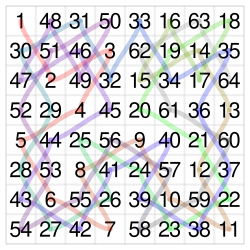
\includegraphics[height=3.6cm]{knight_tour.png}\\
    {\scriptsize Traseu complet pe tablă $8 \times 8$ (numerele indică ordinea mutărilor)}
  \end{center}
\end{frame}

\begin{frame}[fragile]{Traseul calului: implementare cu backtracking}
  \begin{lstlisting}
const int nmax = 8;
int tabla[nmax + 1][nmax + 1];
int dx[] = {-2, -2, -1, -1, 1, 1, 2, 2};
int dy[] = {-1, 1, -2, 2, -2, 2, -1, 1};
int n;

bool valid(int x, int y) {
    return x >= 1 && x <= n && y >= 1 && y <= n
        && tabla[x][y] == 0;
}

void back(int x, int y, int pas) {
    tabla[x][y] = pas;
    if (pas == n * n) {
        // afiseaza tabla[][]
        tabla[x][y] = 0;
        return;
    }
    for (int d = 0; d < 8; d++) {
        int nx = x + dx[d], ny = y + dy[d];
        if (valid(nx, ny)) {
            back(nx, ny, pas + 1);
        }
    }
    tabla[x][y] = 0;       // backtrack
}
// Apel: back(1, 1, 1)
  \end{lstlisting}
\end{frame}

% ==================================================================
\section{Alte aplicații}

\begin{frame}{Backtracking: când este optim și când nu}
  \begin{itemize}
    \item \textbf{Permutări, aranjamente, combinări, submulțimi} $\rightarrow$ backtracking \textbf{optim} (trebuie generate toate soluțiile)
    \item \textbf{N regine, Sudoku, colorarea grafurilor} $\rightarrow$ backtracking cu pruning \textbf{standard}; soluție exponențială inevitabilă
    \item \textbf{Rucsac 0/1:} DP $O(nW)$ când $W$ este mic; \alert{backtracking cu Branch \& Bound} când $W$ este enorm
    \item \textbf{Problema spectacolelor:} backtracking $O(2^n)$, \alert{mai bine greedy $O(n \log n)$}
    \item \textbf{Traseul calului:} backtracking pur, exponențial; \alert{mai bine Warnsdorff $O(n^2)$}
    \item \textbf{Lanț / ciclu hamiltonian, SAT, colorare optimală} $\rightarrow$ probleme \textbf{NP-complete}: backtracking-ul este abordarea clasică
  \end{itemize}
  \begin{block}{Regulă practică}
    Dacă $n \le 20$\textendash{}25, backtracking-ul este viabil. Dacă $n$ este mare, se caută o structură care poate fi exploatată (DP, greedy, Branch \& Bound etc.).
  \end{block}
\end{frame}

\begin{frame}{Rucsac 0/1: Branch \& Bound}
  \begin{block}{Problema}
    Se dau $n$ obiecte cu greutățile $w_i$ și profiturile $p_i$, și un rucsac de capacitate $W$. Se maximizează profitul fără a depăși $W$.
  \end{block}
  \textbf{De ce nu DP?} Complexitatea $O(nW)$ nu este acceptabilă la $W \le 10^9$. Backtracking-ul cu Branch \& Bound evită parcurgerea tuturor celor $2^n$ submulțimi.
  \smallskip

  \textbf{Cele 4 optimizări:}
  \begin{enumerate}
    \item \textbf{sortare} după $p_i / w_i$ descrescător
    \item \textbf{bound optimist:} rucsacul fracționar ca limită superioară
    \item \textbf{inițializare greedy:} un $\mathit{max\_profit}$ bun $\Rightarrow$ pruning agresiv
    \item \textbf{se ia obiectul înainte de a renunța la el}
  \end{enumerate}
  \smallskip
  Dacă $\mathit{profit} + \mathit{bestSuffix}(i, W - \mathit{weight}) \le \mathit{max\_profit}$, ramura se taie (pruning).
\end{frame}

\begin{frame}[fragile]{Rucsac 0/1: implementare Branch \& Bound}
  \lstset{basicstyle=\ttfamily\footnotesize}
  \begin{lstlisting}
// a[i] = {w, p}, sortat dupa p/w descrescator; max_profit initializat greedy
long long weight = 0, profit = 0, max_profit;

long double bestSuffix(int i, long long rem) {
    long double best = 0;
    for (int j = i; j <= n && rem > 0; ++j) {
        long long aux = min(rem, a[j].first);
        best += 1.0L * a[j].second * aux / a[j].first;
        rem -= aux;
    }
    return best;
}

void backtrack(int i) {
    if (i > n) {
        max_profit = max(max_profit, profit);
        return;
    }
    if (profit + bestSuffix(i, W - weight) <= max_profit) {
        return;                              // pruning
    }
    weight += a[i].first;
    profit += a[i].second;
    if (weight <= W) {
        backtrack(i + 1);                    // luam obiectul i
    }
    weight -= a[i].first;
    profit -= a[i].second;
    backtrack(i + 1);                        // nu luam obiectul i
}
  \end{lstlisting}
\end{frame}

\begin{frame}{\texttt{next\_permutation}: generare fără recursivitate}
  \textbf{Ideea:} pentru permutarea curentă se găsește \textit{succesoarea} în ordine lexicografică, până când sunt epuizate toate cele $n!$ permutări.
  \begin{block}{Algoritmul (3 pași)}
    \begin{enumerate}
      \item se găsește cel mai din dreapta $i$ cu $x[i] < x[i+1]$ (sufixul de după $i$ este descrescător)
      \item se găsește cel mai din dreapta $j$ cu $x[j] > x[i]$ și se interschimbă $x[i] \leftrightarrow x[j]$
      \item se inversează sufixul $x[i+1 \ldots n]$
    \end{enumerate}
  \end{block}
  \smallskip
  \textbf{Exemplu:} $(1,3,2) \rightarrow (2,1,3)$
  \begin{itemize}
    \item $x[1] = 1 < x[2] = 3$, deci $i = 1$
    \item cel mai din dreapta $x[j] > 1$ este $x[3] = 2$; interschimbare: $(2,3,1)$
    \item inversarea sufixului $(3,1)$ dă $(2,1,3)$
  \end{itemize}
  \smallskip
  \textbf{Complexitate:} $O(n)$ pe permutare, $O(n \cdot n!)$ în total. \alert{Rezultatul este identic cu cel din backtracking, dar fără stivă recursivă.}
\end{frame}

\begin{frame}[fragile]{\texttt{next\_permutation}: implementare}
  \lstset{basicstyle=\ttfamily\footnotesize}
  \begin{lstlisting}
bool nextPermutation(int x[], int n) {
    int i = n - 1;
    while (i > 0 && x[i] >= x[i + 1]) {
        i--;
    }
    if (i == 0) {
        return false;              // ultima permutare
    }
    int j = n;
    while (x[j] <= x[i]) {
        j--;
    }
    swap(x[i], x[j]);
    int l = i + 1, r = n;          // inversam sufixul x[i+1..n]
    while (l < r) {
        swap(x[l], x[r]);
        l++;
        r--;
    }
    return true;
}

// Generarea tuturor permutarilor lui {1..n}; initial x[i] = i
do {
    for (int i = 1; i <= n; i++) {
        cout << x[i] << " ";
    }
    cout << "\n";
} while (nextPermutation(x, n));
// sau direct: next_permutation(x + 1, x + n + 1)
  \end{lstlisting}
\end{frame}

% ==================================================================
\section{Recapitulare și probleme propuse}

\begin{frame}{Recapitulare}
  \renewcommand{\arraystretch}{1.45}
  \begin{tabular}{@{}p{0.2\textwidth}p{0.17\textwidth}p{0.5\textwidth}@{}}
    \toprule
    \textbf{Obiect} & \textbf{Număr} & \textbf{Ce se schimbă în backtracking} \\
    \midrule
    Permutări & $n!$ & vectorul \texttt{folosit[]}; oprire la $k > n$ \\
    Aranjamente & $\dfrac{n!}{(n-p)!}$ & ca la permutări; oprire la $k > p$ \\
    Combinări & $\dbinom{n}{p}$ & valori strict crescătoare: de la $x[k-1] + 1$ până la $n - p + k$ \\
    Submulțimi & $2^n$ & se extinde cu elemente mai mari, sau include / exclude, sau mască de biți \\
    Produs cartezian & $\displaystyle\prod_k |A_k|$ & fără \texttt{folosit[]}; fiecare poziție are propriul domeniu \\
    \bottomrule
  \end{tabular}
  \smallskip

  Generarea tuturor soluțiilor costă cel puțin numărul lor înmulțit cu lungimea unei soluții; pruning-ul reduce numărul de noduri explorate, dar nu schimbă complexitatea în cel mai rău caz.
\end{frame}

\begin{frame}{Termeni importanți}
  \begin{itemize}
    \item \textbf{Backtracking:} metodă de construire incrementală a unei soluții prin explorarea \textbf{tuturor} posibilităților (DFS în arborele de decizie). La fiecare pas se încearcă toate valorile, după care se \textbf{revine} (\textit{backtrack}) la pasul anterior
    \item \textbf{Arbore de decizie:} structură în care fiecare nod este o stare parțială a soluției, fiecare ramură este o decizie, iar frunzele sunt soluții complete (sau ramuri tăiate)
    \item \textbf{Pruning (tăierea ramurilor):} abandonarea unui subarbore \textbf{imediat ce} se constată că nu poate duce la o soluție validă, fără a-l mai explora. Reduce mult spațiul de căutare la problemele cu constrângeri stricte (N regine, Sudoku)
    \item \textbf{Euristică:} regulă de decizie \textbf{aproximativă} care ghidează căutarea spre soluții bune, fără a garanta optimul. Exemplu: algoritmul lui Warnsdorff pentru traseul calului (se alege celula cu cele mai puține ieșiri libere) funcționează foarte bine în practică, dar nu este demonstrat pentru orice $n$
  \end{itemize}
\end{frame}

\begin{frame}{Probleme propuse: educaționale}
  \large
  \renewcommand{\arraystretch}{1.4}
  \centering
  \begin{tabular}{@{}p{0.5\textwidth}p{0.3\textwidth}@{}}
    \href{https://code.algolymp.com/problems/1704}{\textbf{All Permutations of 1 to N}} & \source{AlgoCode 1704} \\
    \href{https://code.algolymp.com/problems/1705}{\textbf{Cartesian Product Generation}} & \source{AlgoCode 1705} \\
    \href{https://code.algolymp.com/problems/1364}{\textbf{N Queens Board}} & \source{AlgoCode 1364} \\
    \href{https://code.algolymp.com/problems/1373}{\textbf{Arrangements of k Elements}} & \source{AlgoCode 1373} \\
    \href{https://code.algolymp.com/problems/1374}{\textbf{Subsets of k Elements}} & \source{AlgoCode 1374} \\
    \href{https://code.algolymp.com/problems/1375}{\textbf{Nonempty Subsets}} & \source{AlgoCode 1375} \\
    \href{https://code.algolymp.com/problems/1376}{\textbf{Distinct Word Anagrams}} & \source{AlgoCode 1376} \\
    \href{https://code.algolymp.com/problems/1412}{\textbf{Balanced Bracket Strings}} & \source{AlgoCode 1412} \\
  \end{tabular}
\end{frame}

\begin{frame}{Probleme propuse: de antrenament (1/2)}
  \large
  \renewcommand{\arraystretch}{1.4}
  \centering
  \begin{tabular}{@{}p{0.55\textwidth}p{0.3\textwidth}@{}}
    \href{https://code.algolymp.com/problems/1379}{\textbf{Anagrams with Fixed Vowels}} & \source{AlgoCode 1379} \\
    \href{https://code.algolymp.com/problems/1383}{\textbf{Binary Sequences with Same Digit Counts}} & \source{AlgoCode 1383} \\
    \href{https://code.algolymp.com/problems/1386}{\textbf{Constrained Digit Generation}} & \source{AlgoCode 1386} \\
    \href{https://code.algolymp.com/problems/1403}{\textbf{Increasing Sum Decompositions}} & \source{AlgoCode 1403} \\
    \href{https://code.algolymp.com/problems/1404}{\textbf{Signed Squares Equal N}} & \source{AlgoCode 1404} \\
    \href{https://code.algolymp.com/problems/1405}{\textbf{Bounded Banknote Payment}} & \source{AlgoCode 1405} \\
    \href{https://code.algolymp.com/problems/1406}{\textbf{Cube Towers}} & \source{AlgoCode 1406} \\
  \end{tabular}
\end{frame}

\begin{frame}{Probleme propuse: de antrenament (2/2)}
  \large
  \renewcommand{\arraystretch}{1.4}
  \centering
  \begin{tabular}{@{}p{0.55\textwidth}p{0.3\textwidth}@{}}
    \href{https://code.algolymp.com/problems/1411}{\textbf{Distinct Sum Decompositions}} & \source{AlgoCode 1411} \\
    \href{https://code.algolymp.com/problems/1414}{\textbf{Fazan Word Chains}} & \source{AlgoCode 1414} \\
    \href{https://code.algolymp.com/problems/1703}{\textbf{Permutations with Min and Max Fixed}} & \source{AlgoCode 1703} \\
    \href{https://code.algolymp.com/problems/4395}{\textbf{Blocked Queens}} & \source{AlgoCode 4395} \\
    \href{https://code.algolymp.com/problems/1370}{\textbf{Digit Difference Numbers}} & \source{AlgoCode 1370} \\
    \href{https://code.algolymp.com/problems/1706}{\textbf{Special Increasing Sequences}} & \source{AlgoCode 1706} \\
    \href{https://code.algolymp.com/problems/1707}{\textbf{Reciprocal Sum Sequences}} & \source{AlgoCode 1707} \\
  \end{tabular}
\end{frame}

\begin{frame}{Resurse și bibliografie}
  \begin{enumerate}
    \item \textbf{pbinfo.ro} \textemdash{} capitolul „Metoda Backtracking”: teorie, pseudocod și probleme clasice (permutări, regine, labirint)
    \item \textbf{pbinfo.ro} \textemdash{} „Generarea permutărilor / aranjamentelor / combinărilor / submulțimilor”: cod complet pentru fiecare tip de generare
    \item \textbf{GeeksforGeeks} \textemdash{} „Introduction to Backtracking”: arborele de stări, pruning, N-Queens, Sudoku, cu explicații vizuale
    \item \textbf{HackerEarth} \textemdash{} „Recursion and Backtracking”: recursivitatea ca mecanism, backtracking-ul ca strategie, exemplu cu labirint
    \item \textbf{Wikipedia} \textemdash{} „Eight queens puzzle”: 92 de soluții pentru $n = 8$, variante, complexitate
    \item \textbf{Wikipedia} \textemdash{} „Knight's tour”: algoritmul lui Warnsdorff, pătrate magice cu traseu de cal
  \end{enumerate}
\end{frame}

\end{document}
